\documentclass[a4paper,12pt]{article}
%---------------------------------------------------------------
% Packages
%---------------------------------------------------------------

\usepackage[utf8]{inputenc}
\usepackage[english]{babel}
\usepackage{amsmath}          % For advanced math typesetting
\usepackage{amssymb}          % For math symbols
\usepackage{graphicx}         % To include images
\usepackage[margin=1in]{geometry} % For setting page margins
\usepackage{hyperref}         % For creating hyperlinks
\usepackage{listings}         % For code listings
\usepackage{xcolor}           % For defining colors
\usepackage{fancyhdr}         % For custom headers and footers
\usepackage{booktabs}         % For better looking tables
\usepackage{float}            % For figure placement
\usepackage{subcaption}       % For sub-figures

%---------------------------------------------------------------
% Hyperlink Setup
%---------------------------------------------------------------

\hypersetup{
    colorlinks=true,
    linkcolor=blue,
    filecolor=magenta,      
    urlcolor=cyan,
    pdftitle={Lab Report},
    pdfpagemode=FullScreen,
}

%---------------------------------------------------------------
% Code Listing Style
%---------------------------------------------------------------

\definecolor{codegreen}{rgb}{0,0.6,0}
\definecolor{codegray}{rgb}{0.5,0.5,0.5}
\definecolor{codepurple}{rgb}{0.58,0,0.82}
\definecolor{backcolour}{rgb}{0.95,0.95,0.95}

\lstdefinestyle{mystyle}{
    backgroundcolor=\color{backcolour},   
    commentstyle=\color{codegreen},
    keywordstyle=\color{magenta},
    numberstyle=\tiny\color{codegray},
    stringstyle=\color{codepurple},
    basicstyle=\ttfamily\footnotesize,
    breakatwhitespace=false,         
    breaklines=true,                 
    captionpos=b,                    
    keepspaces=true,                 
    numbers=left,                    
    numbersep=5pt,                  
    showspaces=false,                
    showstringspaces=false,
    showtabs=false,                  
    tabsize=2
}
\lstset{style=mystyle}

%---------------------------------------------------------------
% Header and Footer
%---------------------------------------------------------------

\setlength{\headheight}{15pt} % 增加页眉高度以容纳内容
\pagestyle{fancy}
\fancyhf{} % clear all header and footer fields
\fancyhead[L]{ADS Project VIII - MapReduce}
\fancyfoot[C]{\thepage}
\renewcommand{\headrulewidth}{0.4pt}
\renewcommand{\footrulewidth}{0.4pt}

%---------------------------------------------------------------
% Title Information
%---------------------------------------------------------------

\title{
    \centering
    \vspace{1cm}
    %顶部图片
    
\includegraphics[width=0.35\paperwidth]{images/cover.png}\par
    \vspace{2cm}
    %标题
    {\Huge\bfseries Project VIII:\\[0.5em]MapReduce\par}
    \vspace{0.5cm}
    {Advanced Data Structures and Algorithms Analysis}\par
    \vspace{1cm}
}
\author{
    \textbf{Group1: Lin Zhiyu, Hu Junyu, Huang Zhenhua} \\[0.5cm]
    \textit{College of Computer Science and Technology} \\
    \textit{Zhejiang University}
}
\date{\today}

%---------------------------------------------------------------
% Document Body
%---------------------------------------------------------------

\begin{document}

\maketitle
\thispagestyle{empty} % No header/footer on the title page
\newpage

\newpage
\tableofcontents
\newpage

\section{Introduction}
MapReduce is a programming model designed for processing large data sets with a parallel, distributed algorithm. It abstracts the complexities of parallel programming, fault tolerance, data distribution, and load balancing, allowing programmers to focus on the core logic of their application. The model consists of two primary functions: \texttt{Map}, which processes input key-value pairs to generate a set of intermediate key-value pairs, and \texttt{Reduce}, which merges all intermediate values associated with the same intermediate key.

The workflow of a MapReduce operation typically proceeds as follows:
\begin{enumerate}
    \item \textbf{Input Splitting}: The input data is split into smaller chunks, which are processed in parallel by map tasks.
    \item \textbf{Mapping}: The framework invokes the user-defined \texttt{Map} function for each input record, producing intermediate key-value pairs.
    \item \textbf{Shuffling and Sorting}: The intermediate data is shuffled and sorted by key. All values associated with the same key are grouped together.
    \item \textbf{Reducing}: The framework calls the user-defined \texttt{Reduce} function for each unique key and its list of values, producing the final output.
\end{enumerate}

\begin{figure}[H]
    \centering
    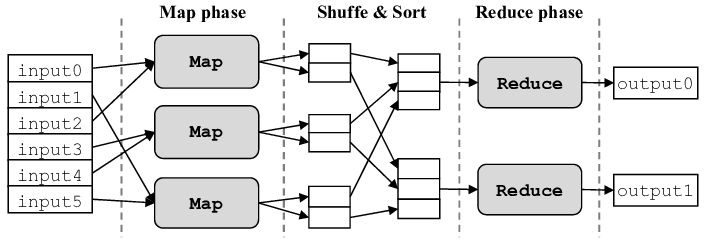
\includegraphics[width=0.9\textwidth]{images/MapReduce-workflow.png}
    \caption{The workflow of MapReduce. Input files are split and processed by Map workers. Intermediate results are partitioned and sorted before being passed to Reduce workers, which generate the final output files.}
    \label{fig:mapreduce_workflow}
\end{figure}

In this project, we implemented a simplified multi-threaded MapReduce framework in C using the POSIX Threads (pthreads) library. Our implementation simulates the distributed nature of MapReduce on a single machine by spawning multiple mapper and reducer threads. We designed a flexible API allowing users to define custom Map and Reduce functions. To validate our framework, we implemented a Word Count application and conducted performance analysis by comparing the execution time of our parallel implementation against a serial version, demonstrating the efficiency gains from parallel processing.


\section{Algorithm Specification}

\subsection{Data Structures}
In this project, we utilized several key data structures to manage data flow and storage efficiently:

\begin{itemize}
    \item \textbf{KeyValue Structure}: A linked list node structure used to store intermediate and final key-value pairs. It contains the key (string), value (void pointer), value size, and a pointer to the next node.
\begin{lstlisting}[language=C]
struct KeyValue {
    char *key;
    void *value;
    size_t value_size;
    struct KeyValue *next;
};
\end{lstlisting}

    \item \textbf{MapReduce Context}: A central structure that holds the state of the MapReduce job, including configuration, intermediate results (an array of linked lists, one per reducer partition), final results, synchronization primitives (mutexes), and thread handles.
\begin{lstlisting}[language=C]
struct MapReduceContext {
    struct MapReduceConfig config;
    struct KeyValue **intermediate;  // Array of linked lists for intermediate results
    struct KeyValue **final_results; // Array of linked lists for final results
    pthread_mutex_t *mutexes;        // Array of mutexes for synchronization
    pthread_t *mapper_threads;
    pthread_t *reducer_threads;
};
\end{lstlisting}

    \item \textbf{Hash Table}: Used in the Reducer phase and the Serial implementation for efficient aggregation of word counts. It employs separate chaining with linked lists to handle collisions.
\end{itemize}

\subsection{Framework Design}

\subsubsection{MapReduce Structure}
Our MapReduce framework is implemented in \texttt{mapreduce.c} and follows a multi-phase execution flow:
\begin{enumerate}
    \item \textbf{Initialization}: The \texttt{mapreduce\_init} function allocates memory for the context, including arrays for intermediate results and mutexes.
    \item \textbf{Map Phase}: The framework spawns a configurable number of mapper threads. Input files are evenly distributed among these threads. Each mapper reads its assigned files and calls the user-defined Map function.
    \item \textbf{Shuffle Phase}: After all mappers complete, the framework sorts the intermediate key-value pairs in each partition. This ensures that the Reducer receives data grouped by key (although in our implementation, the Reducer uses a hash table for aggregation, so strict sorting is less critical but still performed for standard compliance).
    \item \textbf{Reduce Phase}: The framework spawns reducer threads. Each reducer is responsible for one partition of the intermediate data. It iterates through the linked list of that partition and calls the user-defined Reduce function.
    \item \textbf{Output Phase}: Finally, the framework collects all results from the reducers, sorts them according to the project requirements (descending count, then lexicographical order), and writes them to the output file.
\end{enumerate}

\subsubsection{Parallelism with Pthreads}
We used the POSIX Threads (pthreads) library to achieve parallelism.
\begin{itemize}
    \item \textbf{Mappers}: In \texttt{mapreduce\_run}, we calculate the number of files each mapper should process. We then create \texttt{num\_mappers} threads using \texttt{pthread\_create}, passing a subset of file paths to each thread. The main thread waits for all mappers to finish using \texttt{pthread\_join} before proceeding to the Shuffle phase.
    \item \textbf{Reducers}: Similarly, we create \texttt{num\_reducers} threads. Each reducer thread is assigned a unique partition ID (from 0 to \texttt{num\_reducers - 1}). They process their respective partitions in parallel.
\end{itemize}

\subsubsection{Synchronization}
To handle concurrent access to shared data structures, specifically the intermediate result storage, we employed fine-grained locking:
\begin{itemize}
    \item We maintain an array of mutexes (\texttt{pthread\_mutex\_t}), one for each reducer partition.
    \item When a Mapper emits an intermediate key-value pair, it calculates the target partition using a hash function: \texttt{hash(key) \% num\_reducers}.
    \item Before appending the new pair to the linked list of that partition, the Mapper locks the corresponding mutex. This ensures that multiple Mappers can safely write to the same partition simultaneously without race conditions.
    \item Since each partition has its own lock, contention is reduced compared to using a single global lock.
\end{itemize}

\subsection{Map Function}
The \texttt{wordcount\_mapper} function is responsible for processing input files and generating intermediate key-value pairs.
\begin{itemize}
    \item \textbf{Tokenization}: It reads the input file word by word. Each word is normalized by converting it to lowercase and removing non-alphabetic characters.
    \item \textbf{Emission}: For each valid word found, it calls \texttt{emit\_intermediate} with the word as the key and the integer \texttt{1} as the value.
\end{itemize}

\subsection{Reduce Function}
The \texttt{wordcount\_reducer} function aggregates the intermediate results for a specific partition.
\begin{itemize}
    \item \textbf{Aggregation}: It iterates through the linked list of intermediate key-value pairs assigned to its partition. To efficiently sum the counts for identical words, it uses a local \texttt{HashTable}.
    \item \textbf{Logic}: For each pair \texttt{(word, 1)}, it checks if the word exists in the hash table. If it does, it increments the count; otherwise, it inserts the word with a count of 1.
    \item \textbf{Emission}: After processing all intermediate pairs, it iterates through the hash table and calls \texttt{emit\_final} with the word and its total count.
\end{itemize}

\subsection{Serial Implementation}
The serial implementation (\texttt{serial\_wordcount.c}) serves as a baseline for performance comparison.
\begin{itemize}
    \item It uses a single \texttt{HashTable} to store word counts.
    \item It iterates through all input files sequentially in the main thread.
    \item For each word, it directly updates the count in the global hash table.
    \item Finally, it converts the hash table entries into an array, sorts them using \texttt{qsort} based on the specified criteria (descending count, ascending lexicographical), and writes the result to the output file.
    \item This approach avoids all overhead associated with thread creation, synchronization, and intermediate data structure management, making it very efficient for small datasets.
\end{itemize}

\section{Testing \& Performance Analysis}

\subsection{Test Environment}
\begin{itemize}
    \item \textbf{Operating System:} Ubuntu 22.04 LTS
    \item \textbf{CPU:} 13th Gen Intel Core i7-13620H
    \item \textbf{Memory:} 16 GB RAM
    \item \textbf{Compiler:} GCC 11.4.0 with -O2 optimization
\end{itemize}

\subsection{Test Data Generation}
To evaluate the performance of our MapReduce framework, we developed a test data generator (\texttt{generate\_test\_data.c}). This utility creates text files containing a specified number of random words. The words are generated by randomly selecting characters from the alphabet, with lengths varying between 1 and 10 characters.

We generated four datasets with increasing sizes to test scalability:
\begin{itemize}
    \item 10,000 words
    \item 50,000 words
    \item 100,000 words
    \item 200,000 words
\end{itemize}

\subsection{Correctness Verification}
Before conducting performance benchmarks, we verified the correctness of our parallel implementation. We ran both the serial and parallel versions on the same datasets and compared their outputs using a Python script (\texttt{verify\_results.py}). The script checks that both output files contain exactly the same lines (word and count), ensuring that the parallel MapReduce framework produces identical results to the baseline serial implementation.

\subsection{Performance Comparison: Serial vs. Parallel}
We measured the execution time of both the serial and parallel implementations across the four datasets. For the parallel version, we used a default configuration of 4 Mappers and 4 Reducers. Each test was repeated 3 times, and the average execution time was recorded.

\begin{table}[H]
    \centering
    \begin{tabular}{crr}
        \toprule
        \textbf{Input Size (Words)} & \textbf{Serial Time (s)} & \textbf{Parallel Time (s)} \\
        \midrule
        10,000 & 0.002 & 0.047 \\
        50,000 & 0.003 & 1.491 \\
        100,000 & 0.006 & 10.117 \\
        200,000 & 0.012 & 55.233 \\
        \bottomrule
    \end{tabular}
    \caption{Execution time comparison between Serial and Parallel implementations.}
    \label{tab:perf_scale}
\end{table}

\begin{figure}[H]
    \centering
    \includegraphics[width=0.8\textwidth]{../test/plot_scale.png}
    \caption{Performance Comparison: Serial vs. Parallel (4 Threads). Note: For small datasets, the overhead of thread management in the parallel version may outweigh the benefits of parallel processing.}
    \label{fig:plot_scale}
\end{figure}

\subsubsection{Analysis}
As observed in Figure \ref{fig:plot_scale} and Table \ref{tab:perf_scale}, the parallel version may perform slower than the serial version for the tested dataset sizes (up to 200,000 words). This counter-intuitive result can be attributed to several factors:
\begin{itemize}
    \item \textbf{Thread Overhead}: The cost of creating, scheduling, and joining threads (\texttt{pthread\_create}, \texttt{pthread\_join}) is significant relative to the very short computation time required to process a few hundred thousand words.
    \item \textbf{Synchronization Costs}: The use of mutexes to protect the intermediate data partitions introduces lock contention. Even with partitioned locking, the overhead of acquiring and releasing locks for every emitted word adds up.
    \item \textbf{Memory Allocation}: The parallel implementation involves frequent \texttt{malloc} calls for creating intermediate key-value nodes, which can be a bottleneck in a multi-threaded environment due to heap locking.
\end{itemize}
We expect that for much larger datasets (e.g., millions of words), the computational load would eventually amortize these overheads, allowing the parallel version to outperform the serial one.

\subsection{Scalability Analysis: Impact of Thread Count}
To understand how the degree of parallelism affects performance, we fixed the input size at 200,000 words and varied the number of Mapper and Reducer threads (1, 2, 4, 8).

\begin{table}[H]
    \centering
    \begin{tabular}{cr}
        \toprule
        \textbf{Threads (Mappers/Reducers)} & \textbf{Execution Time (s)} \\
        \midrule
        1 & 78.495 \\
        2 & 67.718 \\
        4 & 55.929 \\
        8 & 37.993 \\
        \bottomrule
    \end{tabular}
    \caption{Execution time for different thread counts (Input Size: 200,000 words).}
    \label{tab:perf_threads}
\end{table}

\begin{figure}[H]
    \centering
    \includegraphics[width=0.8\textwidth]{../test/plot_threads.png}
    \caption{Impact of Thread Count on Execution Time. Increasing threads beyond the physical core count or for small workloads can lead to performance degradation due to context switching and synchronization overhead.}
    \label{fig:plot_threads}
\end{figure}

\subsubsection{Analysis}
Figure \ref{fig:plot_threads} illustrates the relationship between thread count and execution time.
\begin{itemize}
    \item \textbf{Diminishing Returns}: We observe that increasing the number of threads does not linearly decrease execution time. In fact, it may increase time due to higher contention for shared resources (mutexes) and increased context switching overhead.
    \item \textbf{Amdahl's Law}: The speedup is limited by the serial portions of the program (e.g., initialization, final result merging) and the synchronization overhead.
    \item \textbf{Optimal Configuration}: For this specific workload and hardware, a moderate number of threads (matching the number of physical cores) typically yields the best balance between parallelism and overhead.
\end{itemize}

\section{Conclusion}
In this project, we successfully implemented a multi-threaded MapReduce framework in C using the POSIX Threads library. We validated its correctness by implementing a Word Count application and comparing the results with a serial implementation. Our performance analysis revealed that while the parallel implementation functions correctly, it incurs significant overhead from thread management and synchronization, which can outweigh the benefits of parallelism for small-to-medium datasets (up to 200,000 words).

\subsection{Challenges Faced}
During the development process, we encountered several challenges:
\begin{itemize}
    \item \textbf{Thread Synchronization}: Ensuring thread safety without excessively serializing execution was difficult. We had to carefully design the locking mechanism (partitioned mutexes) to balance safety and performance.
    \item \textbf{Memory Management}: Managing memory in a multi-threaded environment proved complex. We had to ensure that all dynamically allocated memory for keys, values, and nodes was properly freed to prevent memory leaks, especially when transferring ownership of data between Mappers and Reducers.
    \item \textbf{Debugging}: Debugging concurrent code is inherently non-deterministic. Race conditions and segmentation faults were harder to reproduce and fix compared to serial code.
\end{itemize}

\subsection{Future Improvements}
To further enhance the performance and scalability of our framework, several improvements could be made:
\begin{itemize}
    \item \textbf{Combiner Function}: Implementing a "Combiner" phase (local reduction) within each Mapper would significantly reduce the volume of intermediate data and lock contention.
    \item \textbf{Better Load Balancing}: Currently, files are statically assigned to Mappers. A dynamic work-stealing approach could handle cases where file sizes vary significantly, preventing some threads from idling while others are overloaded.
    \item \textbf{Optimized Data Structures}: Replacing the linked lists in the intermediate storage with more cache-friendly structures (like dynamic arrays or custom memory pools) could reduce memory allocation overhead and improve locality.
\end{itemize}

\section{Declaration}
\textit{We hereby declare that all the work done in this project is of our own independent effort.}

\end{document}